% shared preamble of the theory figures (white background, purple / black theme, sans-serif)
\documentclass[tikz,border=8pt]{standalone}
\usepackage[T1]{fontenc}
\usepackage[scaled=0.92]{helvet}
\renewcommand{\familydefault}{\sfdefault}
\usepackage{amsmath,amssymb}
\usepackage[helvet]{sfmath}
\usetikzlibrary{arrows.meta,calc,decorations.pathreplacing,positioning,backgrounds}
\definecolor{ink}{HTML}{1A1A1F}
\definecolor{cohesin}{HTML}{6A3DE8}
\definecolor{condensin}{HTML}{1BAF7A}
\definecolor{fwd}{HTML}{D1303F}      % CTCF pointing right
\definecolor{rev}{HTML}{2B62D9}      % CTCF pointing left
\definecolor{panel}{HTML}{F8F6FD}
\definecolor{panelline}{HTML}{E3DDF5}
\tikzset{
  fiber/.style={line width=2.1pt,ink,line cap=round,line join=round},
  halo/.style={line width=6pt,white,line cap=round},
  lab/.style={font=\small,text=ink},
  note/.style={font=\footnotesize,text=ink!60},
  hd/.style={font=\bfseries\small,text=ink,anchor=west},
  leader/.style={line width=0.6pt,ink!45},
}
% soft panel, numbered badge, heading
\newcommand{\panelbg}[4]{\draw[rounded corners=9pt,fill=panel,draw=panelline,line width=0.9pt] (#1,#2) rectangle (#3,#4);}
\newcommand{\badge}[3]{\fill[ink] (#1,#2) circle (0.21);\node[white,font=\bfseries\footnotesize] at (#1,#2) {#3};}
% CTCF: a protein on the fibre carrying an arrow that gives the motif direction (f = right, r = left)
\newcommand{\protf}[2]{\draw[rounded corners=3.5pt,line width=0.6pt,draw=fwd!65!black,fill=fwd] (#1-0.3,#2-0.19) rectangle (#1+0.3,#2+0.19);
  \draw[white,line width=1.5pt,-{Stealth[length=3.4pt,width=4.4pt]}] (#1-0.15,#2)--(#1+0.16,#2);}
\newcommand{\protr}[2]{\draw[rounded corners=3.5pt,line width=0.6pt,draw=rev!65!black,fill=rev] (#1-0.3,#2-0.19) rectangle (#1+0.3,#2+0.19);
  \draw[white,line width=1.5pt,-{Stealth[length=3.4pt,width=4.4pt]}] (#1+0.15,#2)--(#1-0.16,#2);}
\newcommand{\prot}[3]{\csname prot#3\endcsname{#1}{#2}}
% ring seen at an angle, drawn as a tube (dark outline, light core); back half and front half
\newcommand{\ringpart}[5]{\draw[line width=4.6pt,#3!80!black,line cap=round] ([shift={(#1,#2)}]#4:0.55 and 0.21) arc[start angle=#4,end angle=#5,x radius=0.55,y radius=0.21];
  \draw[line width=2.4pt,#3!55!white,line cap=round] ([shift={(#1,#2)}]#4:0.55 and 0.21) arc[start angle=#4,end angle=#5,x radius=0.55,y radius=0.21];}
\newcommand{\ringback}[3]{\ringpart{#1}{#2}{#3}{180}{0}}
\newcommand{\ringfront}[3]{\ringpart{#1}{#2}{#3}{180}{360}}
% smooth loop whose foot (ring) is at (cx,y0): half-width W, height H, ring colour
\newcommand{\lloop}[5]{%
  \ringback{#1}{#2}{#5}%
  \draw[fiber] (#1-0.3,#2) .. controls (#1-0.3,#2+0.25*#4) and (#1-#3,#2+0.2*#4) .. (#1-#3,#2+0.55*#4)
     .. controls (#1-#3,#2+0.95*#4) and (#1-0.5*#3,#2+#4) .. (#1,#2+#4)
     .. controls (#1+0.5*#3,#2+#4) and (#1+#3,#2+0.95*#4) .. (#1+#3,#2+0.55*#4)
     .. controls (#1+#3,#2+0.2*#4) and (#1+0.3,#2+0.25*#4) .. (#1+0.3,#2);%
  \ringfront{#1}{#2}{#5}}
% gently undulating fibre from x0 to the loop foot at cx (height y0), and from x1
\newcommand{\base}[4]{%
  \draw[fiber] plot[smooth] coordinates {(#1,0.05) (#1+0.35*#3-0.35*#1,-0.05) (#3-1.4,0.04)} .. controls (#3-0.6,0.02) and (#3-0.3,0.05) .. (#3-0.3,#4);
  \draw[fiber] plot[smooth] coordinates {(#2,-0.05) (#2-0.35*#2+0.35*#3,0.05) (#3+1.4,-0.04)} .. controls (#3+0.6,-0.02) and (#3+0.3,0.05) .. (#3+0.3,#4);}
% stop sign for a blocked leg and a leg arrow
\newcommand{\stopbar}[3]{\draw[#3,line width=2.4pt,line cap=round] (#1,#2-0.2)--(#1,#2+0.2);}
\newcommand{\legarrow}[3]{\draw[cohesin,line width=1.6pt,-{Stealth[length=5pt,width=6pt]},line cap=round] (#1,#3)--(#2,#3);}

\definecolor{A}{HTML}{D1303F}\definecolor{B}{HTML}{5B4FD6}
\tikzset{ln/.style={line width=0.7pt,ink!45},cur/.style={line width=1.8pt,cohesin},thin/.style={line width=0.9pt},
  mv/.style={line width=1.2pt,ink!70,-{Stealth[length=5pt,width=6pt]}},box/.style={rounded corners=5pt,draw=cohesin!70,fill=white,line width=0.9pt,align=center,font=\small,text=ink,inner sep=4pt}}
\begin{document}
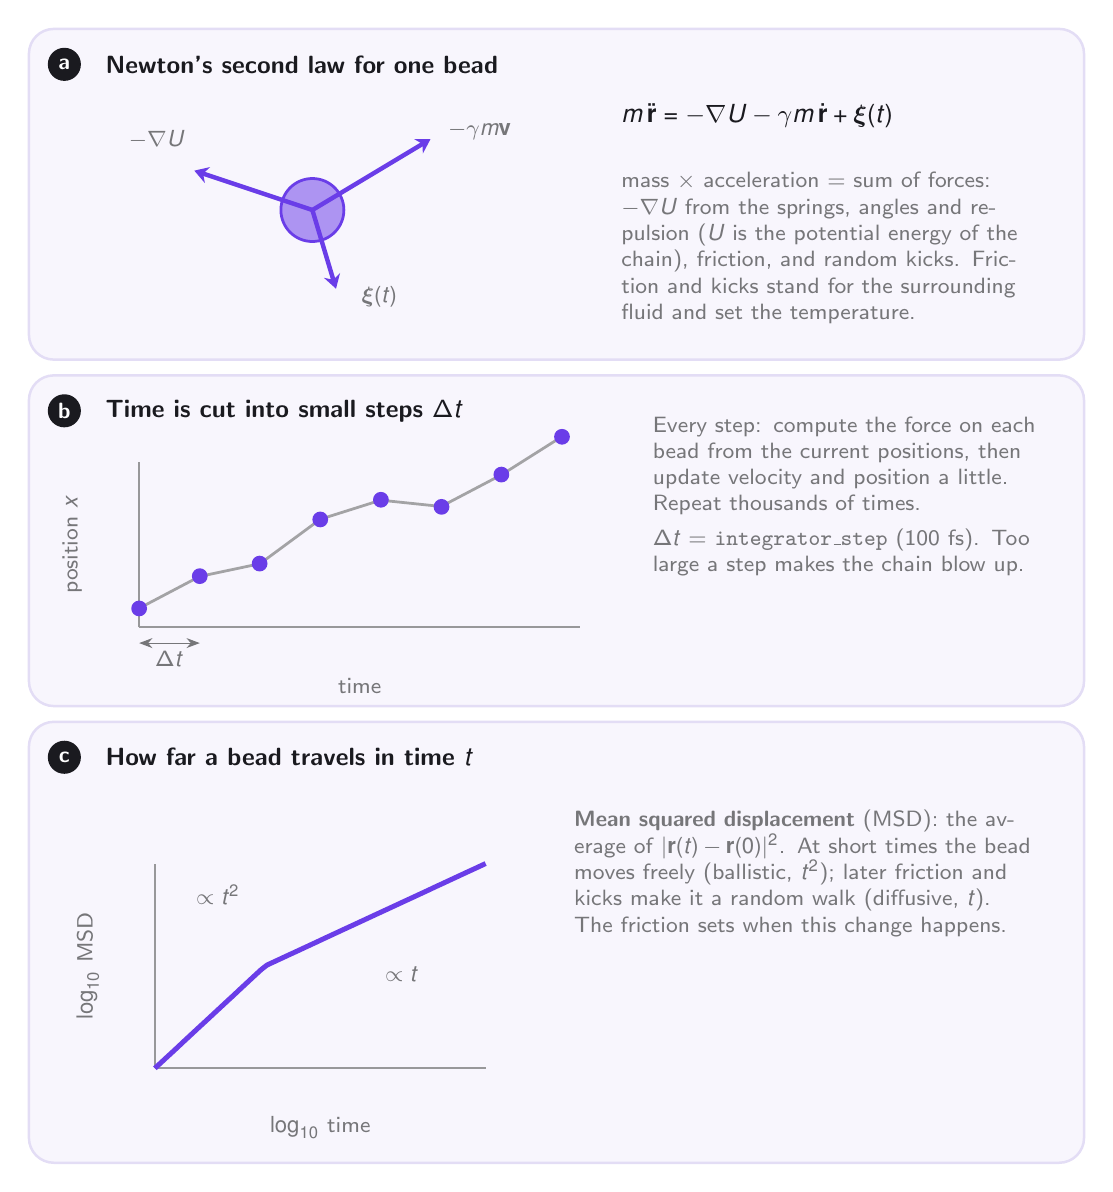
\begin{tikzpicture}
  \panelbg{0}{8.4}{13.4}{12.6}\badge{0.45}{12.15}{a}\node[hd] at (0.85,12.15) {Newton's second law for one bead};
  \panelbg{0}{4.0}{13.4}{8.2}\badge{0.45}{7.749999999999999}{b}\node[hd] at (0.85,7.749999999999999) {Time is cut into small steps $\Delta t$};
  \panelbg{0}{-1.8}{13.4}{3.8}\badge{0.45}{3.3499999999999996}{c}\node[hd] at (0.85,3.3499999999999996) {How far a bead travels in time $t$};
  \fill[cohesin!55] (3.6,10.3) circle (0.4);\draw[cohesin,line width=1pt] (3.6,10.3) circle (0.4);
  \draw[mv,cohesin,line width=1.6pt] (3.6,10.3)--(2.10,10.80);
  \draw[mv,cohesin,line width=1.6pt] (3.6,10.3)--(5.10,11.20);
  \draw[mv,cohesin,line width=1.6pt] (3.6,10.3)--(3.90,9.30);
  \node[note,anchor=east] at (2.1,11.2) {$-\nabla U$};
  \node[note,anchor=west] at (5.2,11.3) {$-\gamma m\mathbf v$};
  \node[note,anchor=west] at (4.1,9.2) {$\boldsymbol\xi(t)$};
  \node[lab,anchor=west] at (7.4,11.5) {$m\,\ddot{\mathbf r}=-\nabla U-\gamma m\,\dot{\mathbf r}+\boldsymbol\xi(t)$};
  \node[note,text width=5.4cm,anchor=north west] at (7.4,10.9) {mass $\times$ acceleration = sum of forces: $-\nabla U$ from the springs, angles and repulsion ($U$ is the potential energy of the chain), friction, and random kicks. Friction and kicks stand for the surrounding fluid and set the temperature.};
  \draw[ln] (1.4,5.0)--(7.0,5.0);\draw[ln] (1.4,5.0)--(1.4,7.1);
  \node[note] at (4.20,4.25) {time};
  \node[note,rotate=90] at (0.55,6.05) {position $x$};
  \draw[line width=1pt,ink!40] plot coordinates {(1.400,5.242) (2.167,5.646) (2.934,5.808) (3.701,6.373) (4.468,6.615) (5.236,6.535) (6.003,6.938) (6.770,7.423)};
  \fill[cohesin] (1.40,5.24) circle (0.1);
  \fill[cohesin] (2.17,5.65) circle (0.1);
  \fill[cohesin] (2.93,5.81) circle (0.1);
  \fill[cohesin] (3.70,6.37) circle (0.1);
  \fill[cohesin] (4.47,6.62) circle (0.1);
  \fill[cohesin] (5.24,6.53) circle (0.1);
  \fill[cohesin] (6.00,6.94) circle (0.1);
  \fill[cohesin] (6.77,7.42) circle (0.1);
  \draw[ink!60,{Stealth}-{Stealth}] (1.40,4.80)--(2.17,4.80);\node[note] at (1.78,4.60) {$\Delta t$};
  \node[note,text width=5.0cm,anchor=north west] at (7.8,7.8) {Every step: compute the force on each bead from the current positions, then update velocity and position a little. Repeat thousands of times.\\[3pt]$\Delta t$ = \texttt{integrator\_step} (100 fs). Too large a step makes the chain blow up.};
  \draw[ln] (1.6,-0.6)--(5.800000000000001,-0.6);\draw[ln] (1.6,-0.6)--(1.6,2.0);
  \node[note] at (3.70,-1.35) {$\log_{10}$ time};
  \node[note,rotate=90] at (0.75,0.70) {$\log_{10}$ MSD};
  \draw[cur] plot coordinates {(1.600,-0.600) (1.671,-0.534) (1.742,-0.468) (1.814,-0.402) (1.885,-0.336) (1.956,-0.269) (2.027,-0.203) (2.098,-0.137) (2.169,-0.071) (2.241,-0.005) (2.312,0.061) (2.383,0.127) (2.454,0.193) (2.525,0.259) (2.597,0.325) (2.668,0.392) (2.739,0.458) (2.810,0.524) (2.881,0.590) (2.953,0.656) (3.024,0.711) (3.095,0.744) (3.166,0.777) (3.237,0.810) (3.308,0.843) (3.380,0.876) (3.451,0.909) (3.522,0.942) (3.593,0.975) (3.664,1.008) (3.736,1.042) (3.807,1.075) (3.878,1.108) (3.949,1.141) (4.020,1.174) (4.092,1.207) (4.163,1.240) (4.234,1.273) (4.305,1.306) (4.376,1.339) (4.447,1.372) (4.519,1.405) (4.590,1.438) (4.661,1.471) (4.732,1.504) (4.803,1.537) (4.875,1.570) (4.946,1.603) (5.017,1.636) (5.088,1.669) (5.159,1.703) (5.231,1.736) (5.302,1.769) (5.373,1.802) (5.444,1.835) (5.515,1.868) (5.586,1.901) (5.658,1.934) (5.729,1.967) (5.800,2.000)};
  \node[note,anchor=west] at (2.0,1.6) {$\propto t^2$};\node[note,anchor=west] at (4.4,0.6) {$\propto t$};
  \node[note,text width=5.8cm,anchor=north west] at (6.8,2.8) {\textbf{Mean squared displacement} (MSD): the average of $|\mathbf r(t)-\mathbf r(0)|^2$. At short times the bead moves freely (ballistic, $t^2$); later friction and kicks make it a random walk (diffusive, $t$). The friction sets when this change happens.};
\end{tikzpicture}
\end{document}
